\documentclass[11pt,a4paper]{article}

\usepackage[T2A]{fontenc}
\usepackage[utf8]{inputenc}
\usepackage[russian]{babel}
\usepackage{amsmath,amssymb}
\usepackage{graphicx}
\usepackage{booktabs}
\usepackage[margin=2.4cm]{geometry}
\usepackage{caption}
\usepackage{enumitem}
\usepackage[hidelinks]{hyperref}
\usepackage{microtype}
% запас растяжения: длинные англоязычные термины иначе вылезают на поля
\emergencystretch=1.5em

\captionsetup{font=small,labelfont=bf}
\setlist{itemsep=2pt,topsep=4pt}

\title{\bfseries На каких токенах применять activation steering\\
\large Natural Language Autoencoder как источник гейтинг-сигнала}
\author{}
\date{Август 2026}

\begin{document}
\maketitle

\begin{abstract}
\noindent
\textbf{Задача.} Activation steering обычно добавляет вектор концепта к активациям
на каждом токене генерации. Это грубо: вмешательство может быть нужно лишь там,
где модель действительно обрабатывает соответствующее свойство. Проверялась
гипотеза, что Natural Language Autoencoder (NLA), переводящий активацию в
текстовое описание, способен указать такие токены.

\textbf{Постановка.} Модель Qwen2.5-3B-Instruct, слой~24 (на нём обучены
доступные веса NLA). Основной концепт --- отказ (refusal); дополнительно
исследованы правдивость и пошаговое рассуждение. Вектор строился методом
разности средних на попарно сопоставленных запросах JailbreakBench;
итоговая оценка --- на held-out наборе XSTest.

\textbf{Метод.} Сравнивались режимы стиринга при \emph{равном бюджете
вмешательства}: на всех токенах, на случайных, на первых~$k$, а также по трём
содержательным гейтам --- проекции на вектор (CAST), линейному классификатору и
латентному представлению NLA. Полезность вмешательства измерялась причинно:
стирился ровно один токен, и фиксировалось изменение исхода.

\textbf{Основные результаты.} (1)~Выбор токена действительно решает очень много:
вмешательство в один удачно выбранный токен даёт 45\,\% исправлений против
3{,}5\,\% у случайного выбора при том же бюджете. (2)~Но для отказа оптимальный
выбор оказался чисто позиционным: полезны только первые три токена, и
содержательные гейты не превосходят контроль, у которого распределение
выбираемых позиций то же, а связь с содержанием разорвана. (3)~Причина
структурная: в однораундовой генерации решение об отказе разрешимо ещё до
первого сгенерированного токена. (4)~Предложена диагностика концептов по моменту
принятия решения. По ней отказ вырожден, а пошаговое рассуждение оказалось
единственной из проверенных постановок, где решение распределено по ответу.
(5)~Сам steering-вектор для NLA нечитаем: reconstruction score $0{,}04$ против
$0{,}74$ у настоящих активаций. (6)~Трижды воспроизвелось расхождение:
офлайн-качество сигнала (AUROC) не предсказывает его причинную пользу для
стиринга.
\end{abstract}

\section{Введение}

Activation steering вмешивается в вычисление модели, добавляя к скрытым
состояниям заранее найденное направление. Приём дёшев и не требует обучения,
поэтому применяется к отказам, правдивости, тональности и другим свойствам.
Стандартная реализация добавляет вектор на \emph{каждом} токене генерации.

Это выглядит расточительным. Допустим, refusal-вектор нужен только там, где
модель формирует отказ. Тогда вмешательство в остальные токены приносит один
побочный ущерб: портит беглость и заставляет отказывать там, где отказывать не
следовало (over-refusal). Отсюда исходный вопрос работы: \emph{на каких токенах
стиринг нужен и можно ли эти токены найти}.

Предлагавшийся инструмент --- Natural Language Autoencoder. NLA переводит
активацию в текстовое описание того, что в ней закодировано, и потому выглядит
естественным детектором: достаточно смотреть, на каких токенах описание говорит
о нужном концепте. Основной риск был назван заранее: steering-вектор --- это
разность активаций, а не активация, и для NLA он может оказаться вне обучающего
распределения.

Работа отвечает на вопрос в три шага. Сначала проверяется, что NLA вообще
осмысленно читает активации выбранной модели. Затем причинно измеряется, какие
токены на самом деле стоит стирить. И наконец режимы гейтинга сравниваются
сквозным прогоном с реальным применением стиринга на отложенном наборе.

Ожидаемого ответа не получилось. Выбор токена действительно важен, но для
отказа он решается позиционно. Ни NLA, ни проекция на вектор, ни классификатор не
обошли простого позиционного контроля. Из этого выросла вторая часть работы:
диагностика, которая заранее показывает, имеет ли вопрос о выборе токенов смысл
для конкретного концепта.

\section{Терминология и методы}

\subsection{Обозначения}

Пусть $x$ --- промпт, а $y_1,\dots,y_T$ --- сгенерированные токены. Через
$a_\ell(t)\in\mathbb{R}^d$ обозначим активацию остаточного потока на слое $\ell$
в позиции, из которой порождается токен $y_t$. Всюду далее $\ell=24$,
$d=2048$; выбор слоя определён доступными весами NLA.

\subsection{Activation steering}

Стиринг с коэффициентом $\alpha$ на множестве шагов $\mathcal{T}\subseteq\{1,\dots,T\}$:
\begin{equation}
a_\ell(t) \leftarrow a_\ell(t) + \alpha\,v,\qquad t\in\mathcal{T},
\label{eq:steer}
\end{equation}
где $v\in\mathbb{R}^d$ --- вектор концепта. Режим $\mathcal{T}=\{1,\dots,T\}$
далее называется \emph{all-token}; любое $\mathcal{T}$ меньшего размера ---
\emph{гейтинг}.

Вектор строится методом разности средних (difference of means) по контрастным
парам: если $\mathcal{P}$ и $\mathcal{N}$ --- множества запросов положительного
и отрицательного класса, то
\begin{equation}
v \;=\; \frac{1}{|\mathcal{P}|}\sum_{x\in\mathcal{P}} a_\ell(x)
      \;-\; \frac{1}{|\mathcal{N}|}\sum_{x\in\mathcal{N}} a_\ell(x).
\label{eq:dim}
\end{equation}
Активация берётся на последнем токене промпта. Этот оценщик предпочтён обученному
классификатору: он устойчивее переносится между распределениями, что в работе
подтвердилось напрямую (раздел~\ref{sec:signals}).

\subsection{Гейт и бюджет вмешательства}

Гейт --- это правило, сопоставляющее токену число $s(t)$ и отбирающее
$\mathcal{T}$ по этому числу. Главное требование к сравнению: \emph{все гейты получают одинаковый бюджет}
$|\mathcal{T}|=k$. Иначе гейтинг выигрывает даром. Он просто реже вмешивается,
и улучшение беглости оказывается артефактом. Поэтому отбор ведётся по $k$ наибольшим значениям $s(t)$
внутри каждого ответа, а не по общему порогу: фиксированный порог давал бы
разным режимам разное число стирённых токенов.

Сравнивались шесть режимов и два контроля:
\begin{itemize}
\item \textbf{all-token} --- вмешательство на всех токенах (бюджет не равен
      остальным, приводится как режим из литературы);
\item \textbf{random} --- $k$ случайных токенов. Обязательный контроль равного
      бюджета;
\item \textbf{first-$k$} --- первые $k$ токенов. Позиционная эвристика;
\item \textbf{cosine} --- $s(t)=\langle a_\ell(t), \hat v\rangle$, проекция на
      вектор. Соответствует подходу conditional activation steering (CAST) и
      является прямым конкурентом;
\item \textbf{probe} --- решающая функция логистической регрессии по активациям;
\item \textbf{NLA-латент} --- см. ниже;
\item \textbf{позиционные контроли} --- см. раздел~\ref{sec:control}.
\end{itemize}

Решение о вмешательстве в токен $t$ принимается по активации $a_\ell(t)$
\emph{до} добавления вектора. Это требование каузальности: иначе гейт видел бы
последствия собственного вмешательства.

\subsection{Natural Language Autoencoder}

NLA --- пара моделей, обученных совместно.

\textbf{Вербализатор} $\mathrm{av}:\mathbb{R}^d\to\Sigma^{*}$ переводит
активацию в текстовое описание. Технически это полная языковая модель:
активация подставляется вместо эмбеддинга специального символа в фиксированном
промпте, после чего модель генерирует объяснение. Никакого масштабирования к
активации не применяется.

\textbf{Реконструктор} $\mathrm{ar}:\Sigma^{*}\to\mathbb{R}^d$ переводит текст
обратно в активацию. Это та же модель, обрезанная до $\ell+1$ слоёв, так что
искомая активация --- выход её последнего блока.

Отсюда естественная мера того, лежит ли вектор в области определения NLA ---
\emph{reconstruction score}:
\begin{equation}
R(a) \;=\; \cos\!\big(a,\ \mathrm{ar}(\mathrm{av}(a))\big).
\label{eq:recon}
\end{equation}
Само по себе это число ничего не значит. В высокой размерности активации одной
модели лежат в общем конусе, поэтому рядом со «своими» парами всегда считаются
«чужие»: объяснение активации $i$ против активации $j\neq i$.

\textbf{Латент.} Текстовая вербализация стоит полной генерации на каждый токен
и для inference непригодна. Поэтому в качестве гейтинг-сигнала использовалось
внутреннее представление $z(a)\in\mathbb{R}^d$ --- скрытое состояние
$\mathrm{av}$ на последней позиции промпта, то есть сводка, с которой
вербализатор подходит к порождению объяснения. Это один forward вместо
шестидесяти. Гейт:
\begin{equation}
s_{\text{NLA}}(t) \;=\; \cos\!\big(z(a_\ell(t)),\ z_{\text{ref}}\big),
\label{eq:nlagate}
\end{equation}
где опора $z_{\text{ref}}$ --- средний латент активаций с наибольшей проекцией
на $v$. Опора строится из хвоста распределения, а не из центроида класса:
усреднение по классу, как показано в разделе~\ref{sec:ood}, стирает различие.

\subsection{Метрики}

\textbf{Отказ.} Подстрочный матчинг по набору формул отказа. Устойчивость
проверена: сужение набора до пяти однозначных формул и расширение до двадцати
трёх, включая мягкие уклонения, не изменили ни одного числа.

Целевые величины --- \emph{over-refusal} (доля отказов на безопасных запросах,
которую надо снизить) и \emph{отказ на опасных} (который надо удержать). Обе
приводятся всегда вместе: улучшение первой при обвале второй означает не
исправление ошибки, а отключение безопасности.

\textbf{Побочный ущерб.} Средний логарифм правдоподобия сгенерированного ответа
\emph{под нестирённой моделью} --- прокси беглости.

\textbf{Правдивость.} Метрика MC2 из работы по TruthfulQA: предпочтение самой
модели между верными и неверными вариантами ответа,
\begin{equation}
\mathrm{MC2}(x) = \log\!\!\sum_{c\,\in\,\text{верные}}\!\!e^{\bar\ell(c\mid x)}
                 -\log\!\!\sum_{c\,\in\,\text{неверные}}\!\!e^{\bar\ell(c\mid x)},
\label{eq:mc2}
\end{equation}
где $\bar\ell(c\mid x)$ --- средний по токенам логарифм вероятности варианта
$c$. Метрика точна по построению: судья не нужен, шума измерителя нет.

\textbf{Момент принятия решения.} Величина, введённая в этой работе для
диагностики концептов. Пусть $m(t)$ --- метрика, вычисленная по промпту и
префиксу из $t$ сгенерированных токенов. Момент фиксации --- наименьшее $t$,
начиная с которого знак $m$ совпадает с итоговым и больше не меняется:
\begin{equation}
t^{*} = \min\{t:\ \operatorname{sign} m(\tau) = \operatorname{sign} m(T)\ \
\forall \tau \ge t\}.
\label{eq:onset}
\end{equation}
Если $t^{*}$ близок к нулю у всех примеров, концепт \emph{front-loaded}: решение
принято до появления содержания, и содержательному гейтингу нечего делать.

\section{Экспериментальная установка}

Модель --- Qwen2.5-3B-Instruct, вычисления в fp16 на одной T4. Веса NLA ---
пара \texttt{rl-v13} для Qwen2.5-3B со слоем~24; у весов нет публичной
документации, интерфейс восстановлен (раздел~\ref{sec:iface}). Пара берётся из
одного обучающего прогона: вербализатор и реконструктор из разных чекпоинтов
дают бессмысленный reconstruction score.

\textbf{Данные для отказа.} Вектор строится на JailbreakBench: 100 вредных и 100
безопасных запросов, попарно сопоставленных по теме и категории. Сопоставление
принципиально --- иначе разность средних выделит тематику, а не вредоносность.
Итоговая оценка --- на XSTest: 150 безопасных запросов, сформулированных так,
что они выглядят опасно, и 150 действительно опасных. \textbf{XSTest не
участвовал ни в построении вектора, ни в выборе позиции извлечения, ни в
калибровке} и использован один раз, для финальной таблицы.

\textbf{Позиция извлечения} выбрана 5-fold кросс-валидацией. Позиции $-1$, $-2$
и $-3$ оказались статистически неразличимы ($0{,}950/0{,}954/0{,}959$ при
стандартном отклонении по фолдам $0{,}023\ldots0{,}037$), поэтому выбор сделан
не по AUROC, а по содержательным доводам: взят последний токен промпта как
стандартная post-instruction позиция с максимальной устойчивостью направления
между фолдами.

\section{Результаты}

\subsection{Интерфейс NLA восстановлен}
\label{sec:iface}

У опубликованных весов нет model card. Формат восстановлен из служебных
метаданных и подтверждён генерацией:

\begin{itemize}
\item вербализатор --- полная 36-слойная модель; реконструктор --- та же
      архитектура, обрезанная до 25 слоёв, то есть активация читается с выхода
      последнего блока;
\item специальных токенов не добавлено: активация подставляется хуком вместо
      эмбеддинга символа U+320E, позиция которого ищется по соседним токенам;
\item нормировочный масштаб из метаданных к активации \textbf{не} применяется.
      Это установлено перебором: без масштабирования объяснения осмысленны на
      всех четырёх пробных активациях, при умножении систематически уходят в
      сторону, при делении вырождаются в мусор. Рассуждение «норма активации
      должна быть сопоставима с нормой эмбеддинга» здесь неверно: отношение норм
      составляет~91;
\item активация --- выход слоя 24, то есть \texttt{hidden\_states[25]} в
      терминах HuggingFace. Выбор между входом и выходом слоя сделан по
      reconstruction score: $0{,}771$ против $0{,}741$.
\end{itemize}

Вербализация работает. Четыре пробные активации (утверждение про Париж, отказ,
определение функции на Python, диагноз пневмонии) дали объяснения точно по своей
теме. Контроль --- активация последнего слоя вместо слоя~24 --- дал набор
мусорных символов, что подтверждает: совпадения не могли возникнуть из промпта.

\subsection{Steering-вектор лежит вне области определения NLA}
\label{sec:ood}

Reconstruction score~\eqref{eq:recon} измерялся на настоящих активациях, на
центроидах классов и на самом векторе.

\begin{table}[htbp]
\centering
\caption{Читаемость разных объектов для NLA. Ориентир: $0{,}74$ --- настоящие
активации, $0{,}52$ --- заведомо чужие пары.}
\label{tab:ood}
\small
\begin{tabular}{lrl}
\toprule
объект & $R$ & о чём объяснение \\
\midrule
центроид вредных запросов & 0{,}736 & «sensitive topic about inappropriate content» \\
центроид безопасных & 0{,}725 & «sensitive topics related to mental health» \\
\textbf{вектор, как есть} & \textbf{0{,}042} & про подарки и кредитные карты \\
\textbf{вектор, нормированный} & \textbf{0{,}053} & про азартные игры \\
безопасный центроид $+\,2v$ & 0{,}663 & «I absolutely condemn any harassment» \\
безопасный центроид $+\,4v$ & 0{,}520 & «We unequivocally condemn Criminal Activity» \\
\bottomrule
\end{tabular}
\end{table}

Голый вектор нечитаем: $0{,}04$ против $0{,}74$ у активаций и $0{,}52$ у чужих
пар, то есть он лежит \emph{дальше случайной чужой активации}. Это ожидаемо: у
разности вычтена та общая компонента, в которой живут все выходы NLA.
Нормирование до типичной длины активации не помогает --- дело в направлении.

Зато \emph{в контексте} направление читается, и с чистой дозовой зависимостью:
по мере роста $\alpha$ объяснения последовательно усиливаются от «чувствительной
темы» до «безоговорочно осуждаем преступную деятельность», а reconstruction
деградирует плавно.

Отдельное наблюдение с прямым следствием для дизайна: центроиды классов описаны
почти одинаково (косинус их реконструкций $0{,}914$), хотя проекция на вектор
разделяет классы с AUROC $0{,}95$. Усреднение по классу стирает
дискриминирующий сигнал, поэтому опора для NLA-гейта строится из хвоста
распределения.

\subsection{Латент NLA несёт концепт, но с потерями}
\label{sec:signals}

Сравнивалось качество разных представлений как признаков для предсказания
отказа, 5-fold кросс-валидация \emph{с разбиением по промптам} (разбиение по
токенам протащило бы один ответ в обучение и тест сразу).

\begin{table}[htbp]
\centering
\caption{Информативность представлений, AUROC на 9561 токене генерации.}
\label{tab:probe}
\small
\begin{tabular}{lr}
\toprule
признаки и способ считывания & AUROC \\
\midrule
классификатор по активации слоя 24 & $0{,}987 \pm 0{,}005$ \\
классификатор по латенту $\mathrm{av}$ & $0{,}954 \pm 0{,}010$ \\
проекция на $v$, без обучения & $0{,}921$ \\
косинус к опорному латенту & $0{,}608$ \\
\bottomrule
\end{tabular}
\end{table}

Информация в латенте есть: $0{,}954$ против $0{,}987$ у сырой активации.
Провал до $0{,}608$ --- свойство наивного считывания, а не латента. Но
существенно и другое: латент \emph{чуть хуже} сырой активации, то есть прогон
через вербализатор --- преобразование с потерями. Признаков того, что NLA видит
нечто, отсутствующее в самой активации, не обнаружено.

Здесь же выяснилось, что обученный классификатор гораздо чувствительнее к
сдвигу распределения, чем разность средних: тот же probe, обученный на
активациях промптов и применённый к активациям генерации, даёт лишь $0{,}61$.

\subsection{Когда концепт фиксируется во времени}
\label{sec:timing}

Момент принятия решения~\eqref{eq:onset} измерен для трёх концептов
(рис.~\ref{fig:timing}).

\begin{figure}[htbp]
\centering
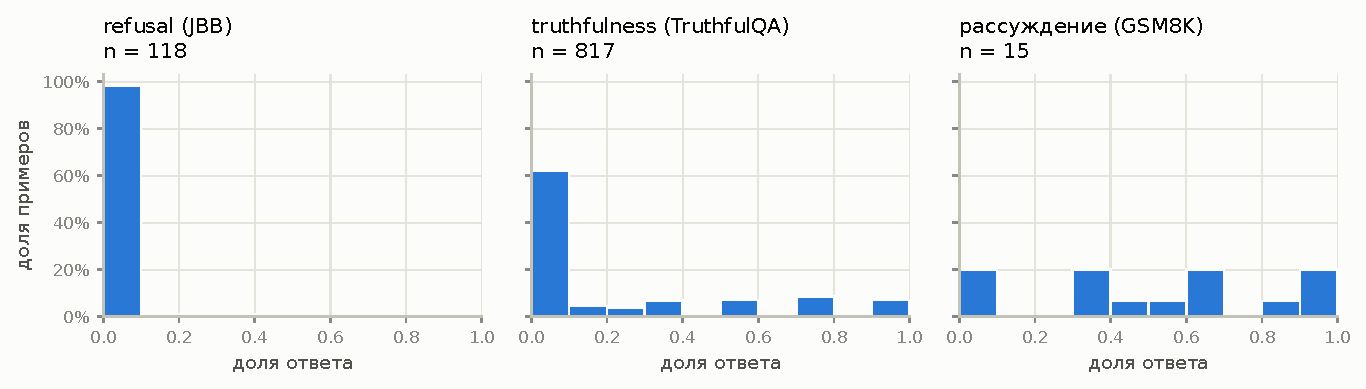
\includegraphics[width=\textwidth]{figures/fig1_timing.pdf}
\caption{Распределение момента фиксации решения, в долях длины ответа. Для
отказа --- позиция первой формулы отказа; для правдивости и рассуждения ---
момент, после которого знак метрики не меняется. Ответы ограничены 48, 32 и 512
токенами соответственно.}
\label{fig:timing}
\end{figure}

Картина резко разная:

\begin{itemize}
\item \textbf{отказ} --- 98\,\% решений в первых 10\,\% ответа, медиана
      $0{,}042$, разброс $0{,}031$. Практически все отказы начинаются на втором
      токене;
\item \textbf{правдивость} --- 62\,\% в первых 10\,\%, но с настоящим хвостом:
      разброс $0{,}315$;
\item \textbf{рассуждение} --- медиана $0{,}513$, то есть \emph{середина
      трейса}, разброс $0{,}320$, в первых 10\,\% лишь 20\,\%.
\end{itemize}

Для отказа вырожденность структурна, а не случайна. В однораундовой генерации
весь запрос лежит в контексте \emph{до} первого сгенерированного токена, поэтому
вопрос «отказывать или нет» всегда разрешим на нулевом шаге. Это подтверждено
отдельной проверкой: составной запрос из двух задач, безопасной и вредной, не
сдвинул момент отказа вовсе (разброс~$0{,}0$) --- модель сначала отказывает и
лишь затем уточняет, к какой из задач это относилось.

\subsection{Причинная карта полезности}
\label{sec:utility}

Какие токены стоит стирить, измерено напрямую: для запросов, на которые модель
ошибочно ответила отказом, вмешательство применялось \emph{ровно в одну позицию}
и фиксировалось, перестал ли ответ быть отказом.

Здесь потребовался неочевидный контроль. Метрика по полному ответу не может дать
положительного результата там, где формула отказа уже произнесена: стиринг на
пятом шаге не убирает «I'm sorry», выданное на втором. Поэтому считалась и
вторая метрика --- отказ по хвосту после стирённой позиции; но и она
интерпретируется лишь после вычитания базового уровня, поскольку маркеры отказа
стоят в начале и хвост чист сам по себе. Рис.~\ref{fig:utility} показывает
результат после вычитания.

\begin{figure}[htbp]
\centering
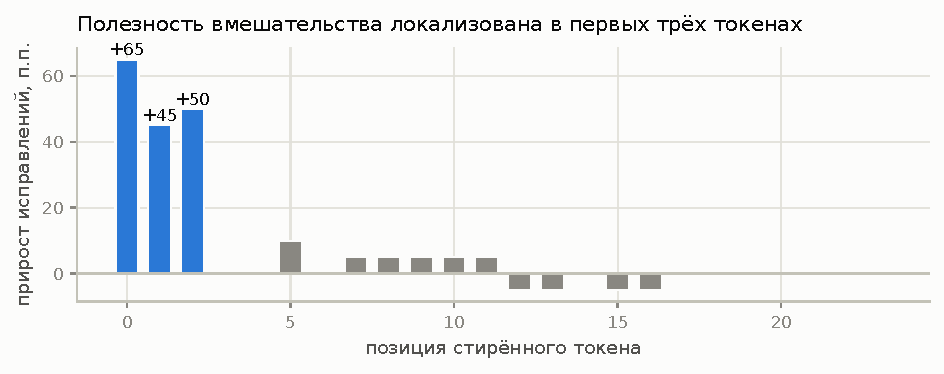
\includegraphics[width=0.92\textwidth]{figures/fig2_utility.pdf}
\caption{Прирост доли исправленных ошибочных отказов при вмешательстве в
единственную позицию, над базовым уровнем. Значимы только позиции 0--2; далее
прирост лежит в пределах $\pm5$ п.п.}
\label{fig:utility}
\end{figure}

Масштаб задают два числа. Вмешательство в один удачно выбранный токен исправляет
45\,\% ошибочных отказов, случайный выбор при том же бюджете --- \textbf{3{,}5\,\%}.
Посылка работы, таким образом, подтверждается причинно: 23 вмешательства из 24
проходят впустую, и от выбора токена зависит почти всё.

Но полезность строго локализована в первых трёх токенах. После вычитания
базового уровня прирост на позициях 3--23 лежит в пределах $\pm5$ п.п., то есть
отсутствует. Оптимальный гейт для отказа, таким образом, чисто позиционный.

\subsection{Сравнение режимов и позиционный контроль}
\label{sec:control}

Итоговое сравнение --- на отложенном XSTest, при равном бюджете $k=2$ и свипе по
силе вмешательства. Свип обязателен: при единственной фиксированной $\alpha$
все режимы обрушивали отказ и на по-настоящему опасных запросах, то есть
отключали отказ вообще, и отличить «гейт бесполезен» от «сила подобрана
неудачно» было невозможно.

\begin{table}[htbp]
\centering
\caption{Режимы гейтинга на held-out XSTest, $k=2$, $\alpha=0{,}5$. Цель ---
снизить over-refusal, удержав отказ на опасных.}
\label{tab:modes}
\small
\begin{tabular}{lrr}
\toprule
режим & over-refusal, \% & отказ на опасных, \% \\
\midrule
без стиринга & 14{,}0 & 80{,}0 \\
\midrule
NLA-латент & 7{,}3 & 72{,}0 \\
\emph{NLA-латент, позиционный контроль} & \emph{7{,}3} & \emph{71{,}3} \\
cosine (CAST) & 11{,}3 & 71{,}3 \\
\emph{cosine, позиционный контроль} & \emph{10{,}7} & \emph{72{,}7} \\
probe & 14{,}0 & 77{,}3 \\
\midrule
первые $k$ & 4{,}7 & 62{,}7 \\
случайные $k$ & 14{,}0 & 76{,}7 \\
все токены & 5{,}3 & 62{,}7 \\
\bottomrule
\end{tabular}
\end{table}

На первый взгляд NLA-латент выигрывает. Он вдвое снижает over-refusal
($14{,}0\to7{,}3$), держит отказ на опасных лучше, чем cosine, и заметно обгоняет
случайный выбор при равном бюджете. Такой вывод и был сделан сначала. Он оказался
неверным.

\textbf{Позиционный конфаунд.} Раздел~\ref{sec:utility} установил, что полезны
только позиции 0--2. Значит гейт, чаще попадающий в этот диапазон, победит без
всякой семантики. Доля таких попаданий: первые~$k$ --- 100\,\%, NLA-латент ---
61{,}5\,\%, cosine --- 39{,}5\,\%, probe --- 15{,}5\,\%, случайный --- 8{,}7\,\%.
Это \emph{в точности} тот порядок, в котором режимы расположились по силе
эффекта (рис.~\ref{fig:confound}). При бюджете в два токена доля позиции~0,
равная 50\,\%, означает, что NLA-латент выбирает нулевой токен почти в каждом
ответе, а cosine --- лишь в 42\,\% ответов.

\begin{figure}[htbp]
\centering
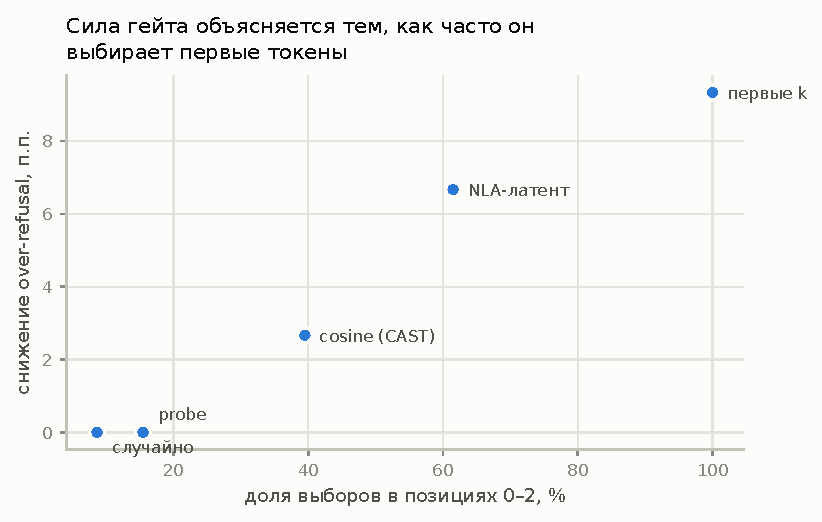
\includegraphics[width=0.78\textwidth]{figures/fig4_confound.pdf}
\caption{Сила гейта как функция того, как часто он выбирает первые три токена.
Точки --- режимы при $\alpha=0{,}5$.}
\label{fig:confound}
\end{figure}

\textbf{Контроль.} Чтобы отделить позицию от содержания, построен контроль
перестановкой: ответу $i$ отдаётся набор позиций, выбранный тем же гейтом для
\emph{другого} ответа $j$. Маргинальное распределение позиций сохраняется в
точности, связь с содержанием разорвана. Такой контроль строже выборки из
маргинала, поскольку сохраняет и структуру набора --- например, «нулевой токен
плюс один поздний».

\begin{figure}[htbp]
\centering
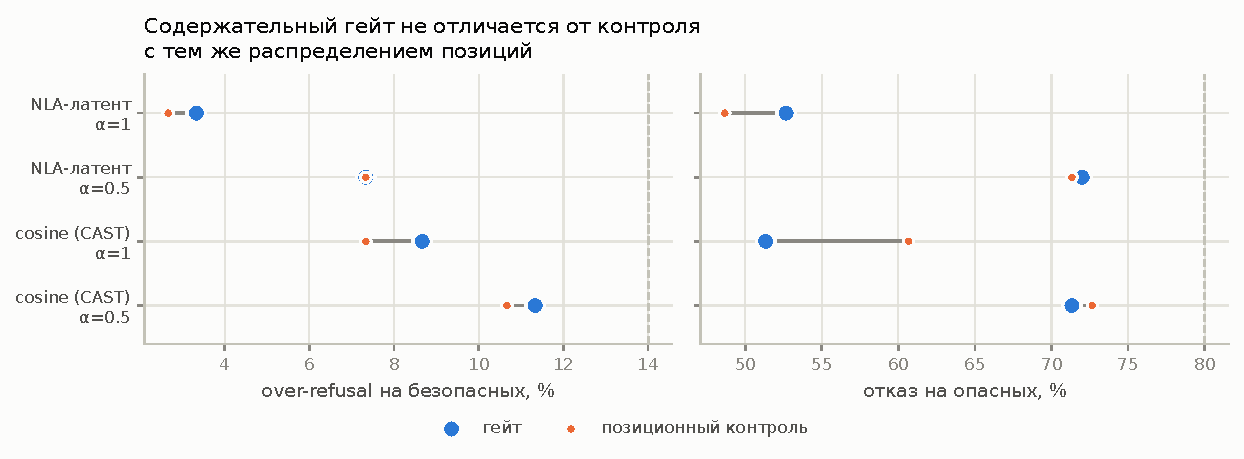
\includegraphics[width=\textwidth]{figures/fig3_control.pdf}
\caption{Гейт против собственного позиционного контроля. Пунктир --- уровень без
стиринга. Значения совпадают либо контроль оказывается лучше.}
\label{fig:control}
\end{figure}

Результат однозначен (рис.~\ref{fig:control}): контроли воспроизводят свои
гейты. У NLA-латента $7{,}3\,\%$ против $7{,}3\,\%$ у контроля; у cosine
контроль даже чуть лучше оригинала ($10{,}7$ против $11{,}3$). При $\alpha=1{,}0$
картина та же, и там контроль cosine превосходит cosine по обеим осям сразу
($7{,}3\,/\,60{,}7$ против $8{,}7\,/\,51{,}3$).

\textbf{Вывод для отказа.} Содержательная информация не даёт ничего: весь эффект
гейта объясняется тем, какие позиции он склонен выбирать. Первоначальный вывод о
превосходстве NLA над проекцией отменяется.

\subsection{Правдивость}
\label{sec:truth}

Поскольку отказ оказался вырожденным, проверялась правдивость --- концепт с
настоящим хвостом в распределении момента решения (раздел~\ref{sec:timing}).

Вектор правдивости строился на контрастных парах утверждений с известной
истинностью, выборка стратифицирована по 12 доменам. Направление выделяется
уверенно: AUROC $0{,}876\pm0{,}038$ при кросс-валидации \emph{по доменам}, то
есть это обобщение истинности, а не запоминание тематики. Формат извлечения
существен: активация из позиции ассистента заметно лучше голого предложения
($0{,}876$ против $0{,}777$).

Однако \emph{перенос на TruthfulQA нулевой}: $0{,}488$ при случайном
уровне~$0{,}5$. И применение вектора ухудшает метрику монотонно
($\rho=-0{,}96$): стиринг «к истине» повышает частоту ошибок на 12{,}7 п.п.

Причину показали проекции. Содержательные верные ответы дают $-1{,}41$, неверные
$-3{,}05$, а \emph{уклончивые верные} --- $-3{,}52$, то есть лежат дальше всех.
Направление, стало быть, отражает \emph{утвердительность высказывания}, а не его
истинность. TruthfulQA же собран из уверенных заблуждений, и треть верных ответов
там уклончива. Это вектор и губит. Полезное следствие: стандартное «truth direction» из литературы на
этом бенчмарке работает в минус.

Проверка альтернативы подтвердила, что дело было в источнике контраста.
Направление, построенное из самой TruthfulQA со сплитом по вопросам, даёт AUROC
$0{,}795$ против $0{,}579$, при косинусе между двумя векторами всего $0{,}086$
--- они почти ортогональны. Заодно проверен слой: 24-й практически оптимален
($0{,}795$ против $0{,}801$ у слоя~30), так что привязка к слою NLA ограничением
не является.

Но и новый вектор не даёт основы для гейтинга (рис.~\ref{fig:truth}).

\begin{figure}[htbp]
\centering
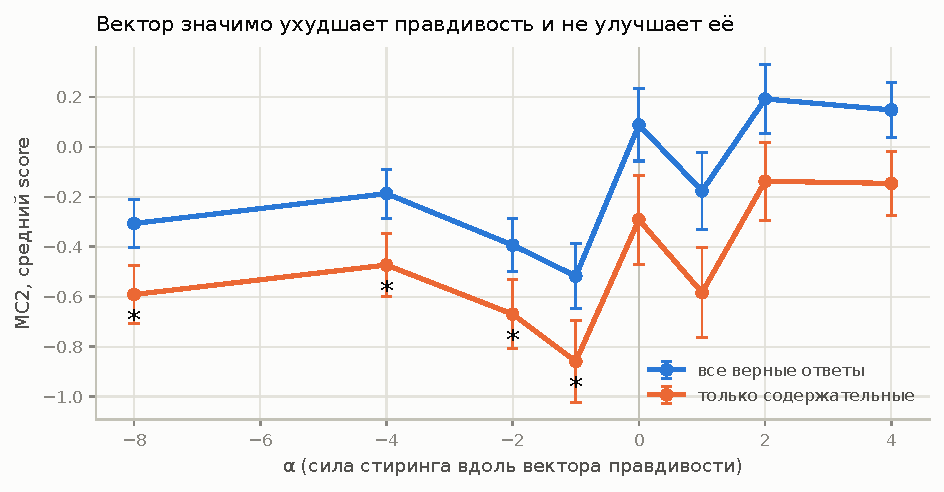
\includegraphics[width=0.92\textwidth]{figures/fig5_truth_alpha.pdf}
\caption{MC2 в зависимости от силы стиринга вдоль вектора, построенного из
TruthfulQA. Усы --- стандартная ошибка среднего; звёздочки --- значимость по
парному критерию Макнемара ($p<0{,}05$).}
\label{fig:truth}
\end{figure}

Парные тесты на 260 вопросах дают асимметричную картину. Отрицательные
$\alpha$ ухудшают метрику \emph{значимо} (до $p=0{,}0000$), то есть направление
обладает настоящей причинной властью. Положительные $\alpha$ значимого улучшения
\emph{не дают}: лучшая точка --- $p=0{,}163$, а после поправки Бонферрони на
перебор семи значений $\alpha$ --- $p=1{,}0$. Монотонность слабая
($\rho=+0{,}64$), и база лучше половины ненулевых точек.

Иными словами, вектором легко \emph{сломать} правдивость и нельзя надёжно её
\emph{починить}. Строить цепочку гейтинга поверх такого направления
бессмысленно: эффекта, который предстояло бы делить между режимами,
статистически нет.

\section{Обсуждение}

\subsection{Офлайн-качество сигнала не предсказывает причинную пользу}

Расхождение воспроизвелось трижды, и дважды привело к неверному промежуточному
выводу, отменённому затем контролем.

\begin{enumerate}
\item По офлайн-AUROC проекция на вектор ($0{,}921$) заметно превосходила
      наивное считывание латента NLA ($0{,}608$). При сквозном прогоне
      NLA-латент оказался \emph{лучше} проекции.
\item Это преимущество, в свою очередь, оказалось позиционным артефактом ---
      обнаружено только контролем с подобранным распределением позиций.
\item Направление правдивости с лучшим разделением ($0{,}795$ против $0{,}579$)
      не дало значимого causal-эффекта, тогда как заметно худшее по AUROC
      направление двигало метрику монотонно и сильно.
\end{enumerate}

Практический вывод простой. AUROC против суррогатной метки удобен, но для отбора
гейтинг-сигнала его мало. Решать следует по причинному измерению.

\subsection{Диагностика концепта как обязательный первый шаг}

Самый переносимый результат работы касается не NLA, а применимости самого
вопроса. Прежде чем строить гейтинг, стоит измерить распределение момента
принятия решения~\eqref{eq:onset}. Когда он сосредоточен в начале ответа, задача
выбора токенов вырождается в позиционную. Содержательный сигнал там бесполезен по
простой причине: решение принято раньше, чем появилось содержание, которое можно
было бы прочитать.

Для однораундового отказа это, по-видимому, свойство постановки, а не модели:
весь запрос доступен до генерации. Концепты, где релевантные события порождает
сама модель по ходу ответа --- в первую очередь пошаговое рассуждение --- этим
свойством не обладают и остаются содержательно интересными.

\section{Ограничения}

Перечислены без смягчений; часть из них прямо ограничивает силу выводов.

\textbf{Текстовый путь NLA не проверен.} Постановка предлагала два
гейтинг-сигнала: текстовые объяснения вербализатора и reconstruction score. Не
использован ни один --- применялся латентный косинус, конструкция производная от
самого вектора. Причина --- стоимость: текстовая вербализация требует полной
генерации на каждый токен, порядка двух десятков минут на тысячу токенов. Поэтому
корректная формулировка вывода --- «данное латентное считывание не превосходит
позиционный контроль», а не «NLA непригоден для гейтинга».

\textbf{Позиционный контроль --- одна перестановка.} Усреднения по нескольким
розыгрышам и доверительного интервала нет. Совпадение $7{,}3$ против $7{,}3$
выглядит убедительно, но формально могло быть удачным розыгрышем.

\textbf{Малые выборки.} База over-refusal 14\,\% на 150 запросах --- это 21
запрос, и обсуждаемые различия суть движение около десяти запросов. Ни одно
парное сравнение режимов не достигло значимости; качественный вывод (контроль
воспроизводит гейт) опирается на воспроизведение при двух значениях $\alpha$, а
не на отдельные проценты. Карта полезности построена на 20 запросах.

\textbf{Один вектор, один сид.} Ресэмплинга вектора и оценки его собственной
изменчивости нет.

\textbf{Гейт офлайновый.} Счёт для токена берётся с нестирённой траектории. Это
каузально корректно и снимает вопрос переноса порогов на сдвинутое
распределение, но означает, что измерен не полностью онлайновый режим: после
вмешательства в нулевой токен активация первого уже другая.

\textbf{Ответы усечены.} В итоговом сравнении --- 32 токена. Отказы возникают
рано, поэтому их детекция корректна, но «согласие» проверено лишь на этом
префиксе.

\textbf{Probe представлен ослабленным.} В итоговой таблице он обучен на
активациях промптов и применён к активациям генерации, из-за чего почти не
отличается от случайного. При обучении на токенах генерации тот же классификатор
даёт AUROC $0{,}987$ (табл.~\ref{tab:probe}), так что как бейзлайн «простого
классификатора» он недооценён.

\textbf{Порог из постановки не построен.} Вместо порогового классификатора над
общим распределением использован отбор $k$ лучших внутри каждого ответа ---
сознательно, ради равного бюджета. Это отличается от буквы задания.

\textbf{Одна модель.} Все выводы получены на Qwen2.5-3B-Instruct и слое~24.
Привязка к слою проверена и оказалась некритичной, привязка к модели --- нет.

\section{Заключение}

Посылка работы подтверждена причинно: выбор токенов для стиринга решает очень
много --- 45\,\% исправлений при удачном выборе против 3{,}5\,\% при случайном
и том же бюджете вмешательства.

Гипотеза о NLA как источнике гейтинг-сигнала на проверенном концепте не
подтвердилась, но подвёл здесь не NLA. Для отказа оптимальный выбор токенов
оказался чисто позиционным. Ни латент NLA, ни проекция на вектор, ни
классификатор не обошли контроля с тем же распределением позиций. Решение об
отказе в однораундовой генерации принимается до появления содержания, так что
интерпретировать попросту нечего.

Попытка перенести вопрос на правдивость упёрлась в отсутствие предпосылки:
доступные направления либо управляют метрикой в неверную сторону, либо ломают её
значимо, не улучшая значимо.

Наиболее переносимый результат --- диагностика концептов по моменту принятия
решения, показывающая, для каких задач вопрос о выборе токенов вообще
содержателен. По этой диагностике пошаговое рассуждение --- единственная из трёх
проверенных постановок, где решение распределено по ответу (медиана на середине
трейса против начала у отказа), метрика точна и измеряет реальный выход модели.
Это и есть естественное продолжение работы. Второе очевидное продолжение ---
текстовый путь NLA, названный в постановке первым и оставшийся непроверенным.

\appendix
\section{Журнал экспериментов}

Все прогоны воспроизводимы: каждой задаче соответствует коммит, зафиксированный
в её логе. Ниже --- сводка; полный журнал с числами и выводами ведётся отдельно.

\begin{table}[htbp]
\centering
\small
\caption{Сводка экспериментов. Отменённые выводы оставлены в журнале намеренно:
они показывают, где контроль поймал ошибку.}
\begin{tabular}{llp{7.6cm}}
\toprule
\# & предмет & исход \\
\midrule
00--01 & интерфейс NLA & восстановлен, подтверждён генерацией \\
02 & масштаб и выбор тензора & масштаб не применяется; активация --- выход слоя 24 \\
03 & reconstruction score & выбор тензора подтверждён количественно \\
04 & вектор отказа & AUROC 0{,}95 на JBB и XSTest \\
04b & позиция извлечения & позиции $-1/-2/-3$ неразличимы, выбор по доводам \\
05 & NLA на векторе и центроидах & вектор нечитаем ($0{,}04$); центроиды неразличимы \\
06--07 & сигналы на токенах генерации & латент несёт концепт с потерями \\
07b & информативность представлений & $0{,}954$ против $0{,}987$; ранний вывод отменён \\
08 & карта полезности & полезны только позиции 0--2 \\
08b & базовый уровень карты & метрика по хвосту требует вычитания базы \\
09 & составные запросы & отрицательный: отказ front-loaded структурно \\
10--10b & пилот правдивости & метрика-классификатор негодна ($58{,}6\,\%$) \\
10c--10d & пилот на правдоподобии & 41\,\% вопросов с поздней фиксацией \\
11 & пилот рассуждения & самая невырожденная постановка \\
12 & сравнение режимов & вывод о превосходстве NLA \emph{отменён} \\
13 & верификация & числа сходятся; найден позиционный конфаунд \\
12b & позиционный контроль & содержательный гейт равен контролю \\
14--18 & правдивость & вектор ломает значимо, не чинит значимо \\
\bottomrule
\end{tabular}
\end{table}

\section{Воспроизведение}

Тяжёлые вычисления выполнялись на бесплатном Colab с T4, локально --- только
анализ агрегатов. Обмен шёл через очередь задач на Google~Drive: код доставлялся
git-синхронизацией, артефакты возвращались на Drive. Каждая долгая задача
кэширует фазы, поэтому обрыв сессии не стоит пересчёта; прогресс пишется в
отдельный файл, поскольку основной лог, удерживаемый открытым, синхронизируется
рывками.

\end{document}
